%%%%%%%%%%%%%%%%%%%%%%%%%%%%%%%%%%%%%%%%%%%%%%%%%%%%%%%%%%%%%%%%%%%%%%%%%%%%%%%%%%%%%%%%%%%%%%%%%%%%%%%%%%%%%%%%%%%%%%%%%%%%%%%%%%%%%%%%%%%%%%%%%%%%%%%%%%%%%%%%%%%
% Written By Michael Brodskiy
% Class: Circuits & Signals: Biomedical Applications
% Professor: N. Sun
%%%%%%%%%%%%%%%%%%%%%%%%%%%%%%%%%%%%%%%%%%%%%%%%%%%%%%%%%%%%%%%%%%%%%%%%%%%%%%%%%%%%%%%%%%%%%%%%%%%%%%%%%%%%%%%%%%%%%%%%%%%%%%%%%%%%%%%%%%%%%%%%%%%%%%%%%%%%%%%%%%%

\documentclass[12pt]{article} 
\usepackage{alphalph}
\usepackage[utf8]{inputenc}
\usepackage[russian,english]{babel}
\usepackage{titling}
\usepackage{amsmath}
\usepackage{graphicx}
\usepackage{enumitem}
\usepackage{amssymb}
\usepackage[super]{nth}
\usepackage{everysel}
\usepackage{ragged2e}
\usepackage{geometry}
\usepackage{multicol}
\usepackage{fancyhdr}
\usepackage{cancel}
\usepackage{siunitx}
\usepackage{physics}
\usepackage{tikz}
\usepackage{mathdots}
\usepackage{yhmath}
\usepackage{cancel}
\usepackage{color}
\usepackage{array}
\usepackage{multirow}
\usepackage{gensymb}
\usepackage{tabularx}
\usepackage{extarrows}
\usepackage{booktabs}
\usetikzlibrary{fadings}
\usetikzlibrary{patterns}
\usetikzlibrary{shadows.blur}
\usetikzlibrary{shapes}

\geometry{top=1.0in,bottom=1.0in,left=1.0in,right=1.0in}
\newcommand{\subtitle}[1]{%
  \posttitle{%
    \par\end{center}
    \begin{center}\large#1\end{center}
    \vskip0.5em}%

}
\usepackage{hyperref}
\hypersetup{
colorlinks=true,
linkcolor=blue,
filecolor=magenta,      
urlcolor=blue,
citecolor=blue,
}


\title{Fourier Series}
\date{\today}
\author{Michael Brodskiy\\ \small Professor: N. Sun}

\begin{document}

\maketitle

\begin{itemize}

  \item Periodic Signals

    \begin{itemize}

      \item Sinusoidal signals are periodic

      \item A periodic function is a function that repeats itself after $T$ seconds

    \end{itemize}

  \item Fourier Series

    \begin{itemize}

      \item The Fourier series representation of a periodic signal is:

        $$\boxed{f(t)=a_0+\sum_{n=1}^{\infty} a_n\cos(n\omega_0t)+b_n\sin(n\omega_0t)}$$

      \item The coefficients may be determined in the following manner:

        $$a_0=\frac{1}{T}\int_0^T f(t)\,dt$$

        $$a_k=\frac{2}{T}\int_0^T f(t)\cos(k\omega_0t)\,dt$$

        $$b_k=\frac{2}{T}\int_0^T f(t)\sin(k\omega_0t)\,dt$$

        \begin{itemize}

          \item Even though the indicated limits of integration are from 0 to $T$, the expressions are equally valid if the lower limit is changed to $t_0$ and the upper limit to $(t_0+T)$ for any value of $t_0$; in some cases, the evaluation is easier to perform by integrating from $-\dfrac{T}{2}$ to $\dfrac{T}{2}$

          \item For an even function $(f(t)=f(-t))$:

            $$a_0=\frac{2}{T}\int_0^{\frac{T}{2}}f(t)\,dt$$

            $$a_k=\frac{4}{T}\int_0^{\frac{T}{2}}f(t)\cos(k\omega_0t)\,dt$$

            $$b_k=0$$

          \item For an odd function $(f(t)=-f(-t))$:

            $$a_0=0$$

            $$a_k=0$$

            $$b_k=\frac{4}{T}\int_0^{\frac{T}{2}}f(t)\sin(k\omega_0t)\,dt$$

        \end{itemize}

    \end{itemize}

  \item Some common Fourier transforms are:

  \begin{center}
    \begin{figure}[h!]
      \centering
      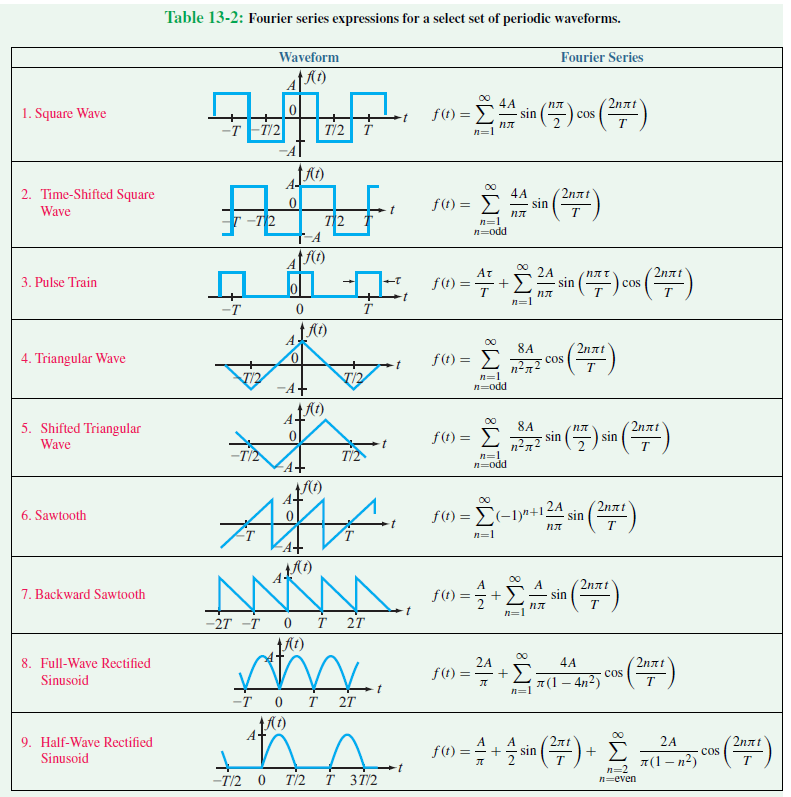
\includegraphics[width=.65\textwidth]{Figures/FT.png}
      \caption{Common Fourier Transform Table}
      \label{fig:1}
    \end{figure}
  \end{center}

\end{itemize}

\end{document}

